% This is samplepaper.tex, a sample chapter demonstrating the
% LLNCS macro package for Springer Computer Science proceedings;
% Version 2.20 of 2017/10/04
%
\documentclass[runningheads]{llncs}
%
\usepackage{graphicx}
\usepackage{caption}
\usepackage{subcaption}
% \usepackage{pdfpages}
% Used for displaying a sample figure. If possible, figure files should
% be included in EPS format.
%
% If you use the hyperref package, please uncomment the following line
% to display URLs in blue roman font according to Springer's eBook style:
% \renewcommand\UrlFont{\color{blue}\rmfamily}

% % Dãn dòng 1.5
% \usepackage{setspace}
% \onehalfspacing

% Font tiếng Việt
\usepackage[T5]{fontenc}
\usepackage[utf8]{inputenc}
\DeclareTextSymbolDefault{\DH}{T1}

% Chèn và định dạng mã giả
\usepackage{amsmath}
\usepackage{algorithm}
\usepackage[noend]{algpseudocode}
\makeatletter
\def\BState{\State\hskip-\ALG@thistlm}
\makeatother

% chèn inline code
\usepackage{xparse}
\NewDocumentCommand{\codeword}{v}{%
    \texttt{\textcolor{blue}{#1}}%
}

% equation
\usepackage{breqn}
\usepackage{amsfonts}
\usepackage{bm}

% Bảng biểu
\usepackage{multirow}
\usepackage{float}
\usepackage{makecell}
\usepackage{rotating}
\usepackage{vcell}
\usepackage{array}
\usepackage{diagbox}
\usepackage{booktabs}
\usepackage{colortbl}
\newcolumntype{L}[1]{>{\raggedright\let\newline\\\arraybackslash\hspace{0pt}}m{#1}}
\newcolumntype{C}[1]{>{\centering\let\newline\\\arraybackslash\hspace{0pt}}m{#1}}
\newcolumntype{R}[1]{>{\raggedleft\let\newline\\\arraybackslash\hspace{0pt}}m{#1}}

\begin{document}
%
\title{Meta-learning and Personalization layer \\in Federated learning}
%
% \titlerunning{Abbreviated paper title}
% If the paper title is too long for the running head, you can set
% an abbreviated paper title here
%
\author{Bao-Long Nguyen\inst{1}\orcidID{0000-0002-6411-8943} \\\and
Tat-Cuong Cao\inst{1}\orcidID{0000-0003-1803-843X}}
%
% \authorrunning{F. Author et al.}
% First names are abbreviated in the running head.
% If there are more than two authors, 'et al.' is used.
%
\institute{VNU HCM University of Science, Ho Chi Minh City 749000, Vietnam}
%
\maketitle              % typeset the header of the contribution
%
\begin{abstract}
Khái niệm \textit{Federated Learning} (FL) cùng thuật toán \textit{Federated Averaging} ra đời, được xem như một giải pháp thay thế cho huấn luyện tập trung. Giải pháp này không những đạt hiệu quả gần như tương đương các phương pháp học sâu đã có, giải quyết được vấn đề chi phí phần cứng, mà còn đảm bảo được quyền riêng tư dữ liệu người dùng. Tuy nhiên, đứng trước dữ liệu không đồng nhất và có tính cá nhân hóa cao trên từng người dùng (dữ liệu Non-IID), hệ thống này bị suy giảm hiệu suất nghiêm trọng \cite{zhao2018federated}. Nghiên cứu cải thiện hiệu suất và tăng tính cá nhân hoá của hệ thống FL trên dữ liệu Non-IID bằng thuật toán \codeword{FedMeta-Per} - sự kết hợp giữa phương pháp huấn luyện meta-learning \cite{hospedales2020meta} và kỹ thuật personalization layer \cite{zhu2021federated} vào hệ thống FL.

\keywords{Federated learning \and Non-IID \and Meta-learning \and Personalization layer.}
\end{abstract}
%
%
%

\section{Introduction}

Trong kỷ nguyên Internet of Things (IoT), đứng trước một lượng dữ liệu khổng lồ tại các thiết bị biên được sinh ra mỗi giây, quá trình huấn luyện tập trung bộc lộ nhiều nhược điểm. Thứ nhất, dữ liệu tại các thiết bị biên thường hám chứa những thông tin nhạy cảm về người dùng. Khi phải truyền về một máy chủ để huấn luyện, các thông tin này có thể bị lộ, ảnh hưởng nghiêm trọng đến quyền riêng tư dữ liệu. Thứ hai, chi phí truyền tin giữa máy chủ và các máy khách rất tốn kém do phải truyền một lượng lớn dữ liệu về máy chủ. Thứ ba, máy chủ phải có khả năng tính toán và lưu trữ lớn để tiến hành quá trình huấn luyện.

Tính toán biên \cite{khan2019edge} ra đời nhằm đẩy quá trình tính toán và lưu trữ dữ liệu từ máy chủ đến các máy khách hay thiết bị biên, giúp giảm tải cho máy chủ. Hơn nữa, việc tính toán được chuyển đến gần hoặc ngay tại nơi sản sinh dữ liệu, giúp tiết kiệm một lượng lớn chi phí truyền tin và giảm độ trễ khi tính toán. Không những thế, quá trình trao đổi dữ liệu giữa máy chủ và máy khách không còn diễn ra, giúp tăng đáng kể quyền riêng tư dữ liệu của người dùng.

Trên tinh thần của tính toán biên, \textit{federated learning} (FL) \cite{mcmahan2017communication} ra đời, nhằm huấn luyện mô hình máy học trên các tập dữ liệu riêng biệt, được phân bố trên các thiết bị biên \cite{yin2021comprehensive}. Cụ thể, mục tiêu của hệ thống FL là tìm kiếm một tham số toàn cục $w_G^*$ sao cho độ lỗi của hệ thống đạt cực tiểu:

\begin{dmath}
    w_G^* = \arg\min_{w_G}{f_{global}(w_G)}
        = \arg\min_{w_G}{\frac{1}{n} \sum_{i=1}^n{f_{local}(w_i)}}
\end{dmath} Trong đó, $n$ là số máy khách tham gia vào hệ thống, $f_{global}$ là độ lỗi của toàn hệ thống, $f_{local}(w_i)$ là độ lỗi của máy khách $i$ khi sử dụng tham số $w_i$. 

Phương pháp huấn luyện này không những thừa hưởng những lợi ích từ quá trình tính toán biên (chi phí phần cứng và độ trễ giảm, bảo mật dữ liệu tăng) mà còn có khả năng tăng tính cá nhân hoá cho từng người dùng. Tuy nhiên, các máy khách tham gia vào hệ thống thường không đồng nhất về khả năng lưu trữ và tính toán. Dữ liệu phân bố trên các máy khách này cũng không mang một phân phối giống nhau (non-IID). Điều này tạo ra hai vấn đề chính của một hệ thống FL: Thách thức về hệ thống và Thách thức về thống kê \cite{li2020federated}. Đối với vấn đề thống kê, nghiên cứu \cite{zhao2018federated} chỉ ra rằng thuật toán truyền thống của FL - Federated Averaging (\codeword{FedAvg}) bị giảm hiệu suất nghiêm trọng trên dữ liệu non-IID. Nghiên cứu này nhằm giải quyết một phần vấn đề thống kê. Cụ thể, nghiên cứu tập trung vào cải thiện hiệu suất cũng như tính cá nhân hoá trong việc dự đoán trên dữ liệu non-IID.

Trong nghiên cứu này, chúng tôi cải thiện hiệu suất của hệ thống FL trên dữ liệu non-IID bằng meta-learning (ML) \cite{hospedales2020meta} và kỹ thuật personalization layer (PL). Các thuật toán ML theo hướng tối ưu hai cấp độ có thể tạo ra một khởi tạo có khả năng thích ứng nhanh trên nhiệm vụ mới. Việc sử dụng các thuật toán ML trong huấn luyện nhằm thu được một tham số toàn cục có khả năng thích ứng nhanh trên tập dữ liệu mới của từng người dùng. Trong khi đó, việc sử dụng các kỹ thuật PL để duy trì một phần mạng học sâu tại các thiết bị biên giúp cải thiện hơn nữa tính cá nhân hoá.

\textbf{Đóng góp chính}. Nghiên cứu đề xuất thuật toán \codeword{FedMeta-Per}, một sự kết hợp giữa các thuật toán ML (\codeword{MAML} \cite{finn2017model}, \codeword{Meta-SGD} \cite{li2017meta}) và các kỹ thuật PL (\codeword{FedPer} \cite{arivazhagan2019federated}, \codeword{LG-FedAvg} \cite{liang2020think}), giúp làm tăng độ chính xác lẫn tính cá nhân hoá trên từng người dùng. Qua thực nghiệm, nghiên cứu chỉ ra tính hiệu quả trong việc tăng độ chính xác cũng như tính cá nhân hoá của của thuật toán đề xuất so với thuật toán \codeword{FedAvg}, các thuật toán có sự kết hợp của ML vào FL \cite{chen2018federated} (\codeword{FedMeta(MAML)}, \codeword{FedMeta(Meta-SGD)}) và thuật toán sử dụng PL (\codeword{FedPer}) trên hệ thống FL gồm 50 người dùng, lần lượt chứa dữ liệu của hai tập dữ liệu CIFAR-10 \cite{krizhevsky2009learning} và MNIST \cite{deng2012mnist}.

\section{Related Work}

Từ khi thuật toán \codeword{FedAvg} được giới thiệu lần đầu vào năm 2017, tới nay, đã có rất nhiều công trình được đưa ra nhằm cải thiện độ chính xác của hệ thống trên dữ liệu non-IID. Tại đây, nghiên cứu điểm qua một vài công trình tiêu biểu trong việc thực hiện mục tiêu này.

% \textbf{Sử dụng dữ liệu}. Nếu thiếu trang sẽ viết thêm

% \textbf{Sử dụng nhiều máy chủ}. Nếu thiếu trang sẽ viết thêm

\textbf{Sử dụng meta-learning}. ML là một phương pháp học mới, cho phép mô hình học có thể gia tăng kinh nghiệm qua việc thực hiện nhiều nhiệm vụ khác nhau trong cùng một phân phối nhiệm vụ. Dẫn đến việc các mô hình ML có khả năng thích ứng nhanh trên nhiệm vụ mới chỉ sau một vài bước huấn luyện với dữ liệu huấn luyện giới hạn. Đây là một phát kiến quan trọng, đóng vai trò trong việc đưa cách học tập của máy trở nên tiệm cận với cách học tập của con người \cite{harlow1949formation}.

% Cụ thể, trong cài đặt của ML cho bài toán học có giám sát, tập dữ liệu huấn luyện và kiểm tra lần lượt là $\mathcal{D}_{train} = \{ ( \mathcal{D}_{train(i)}^{support}, \mathcal{D}_{train(i)}^{query} ) \}_{i=1}^{|\mathcal{D}_{train}|}$ và $\mathcal{D}_{test} = \{ ( \mathcal{D}_{test(i)}^{support}, \mathcal{D}_{test(i)}^{query} ) \}_{i=1}^{|\mathcal{D}_{test}|}$. Mỗi phần tử trong các tập dữ liệu trên bao gồm tập support và query và đại diện cho một nhiệm vụ. Theo đó, 

Trong ngữ cảnh dữ liệu non-IID, mỗi người dùng, với nhu cầu khác nhau, sinh ra các tập dữ liệu có phân phối rất khác nhau. Nếu coi mỗi người dùng là một nhiệm vụ, việc huấn luyện mô hình toàn cục trên một tập hợp người dùng của FL sẽ tương đương với việc huấn luyện mô hình máy học trên một phân phối nhiệm vụ của ML. Nghiên cứu \cite{chen2018federated} đề xuất framework \codeword{FedMeta} và minh hoạ thực nghiệm bằng hai thuật toán \codeword{FedMeta(MAML)}, \codeword{FedMeta(Meta-SGD)}. Kết quả cho thấy mô hình toàn cục có khả năng thích ứng nhanh, hội tụ nhanh hơn \codeword{FedAvg} trên tập dữ liệu LEAF \cite{caldas2018leaf}. Nghiên cứu \cite{fallah2020personalized} đề xuất kết hợp \codeword{MAML} trên tập dữ liệu CIFAR-10 và nghiên cứu \cite{jiang2019improving} đề xuất kết hợp \codeword{Reptile} \cite{nichol2018first} trên tập dữ liệu EMNIST-62 vào hệ thống FL để tăng tính cá nhân hoá trên từng máy khách.

Mặt khác, một hệ thống FL, theo thời gian sẽ có sự xuất hiện của các máy khách mới. Một điểm trừ cho các hệ thống sử dụng ML trong huấn luyện là chúng đối xử như nhau với những máy khách đã tồn tại lâu trong hệ thống và những máy khách vừa tham gia vào hệ thống. Do đó, dù mô hình toàn cục có khả năng thích ứng nhanh trên dữ liệu mới, hiệu năng của chúng hoàn toàn có thể được cải thiện thêm.

\textbf{Sử dụng personalization layer}. Để nắm bắt được đặc tính dữ liệu, vốn mang tính cá nhân hoá cao trên từng người dùng khác nhau, việc duy trì một phần mạng học sâu tại các máy khách (được gọi là phần riêng) được đề xuất. Theo đó, nghiên cứu \cite{arivazhagan2019federated} đề xuất thuật toán \codeword{FedPer} với ý tưởng duy trì các lớp fully-connected của mạng học sâu tại máy khách với mục tiêu tăng tính cá nhân hoá. Thực nghiệm cho thấy, \codeword{FedPer} đạt kết quả cao hơn rất nhiều so với \codeword{FedAvg} khi thử nghiệm trên các tập dữ liệu CIFAR-10 và CIFAR-100. Bên cạnh đó, nghiên cứu \cite{liang2020think} với thuật toán \codeword{LG-FedAvg} đề xuất duy trì các lớp rút trích đặc trưng của mạng học sâu tại các máy khách với mục tiêu nắm bắt được các đặc trưng của từng máy khách khác nhau. Kết quả thu được thậm chí còn tốt hơn \codeword{FedPer} trong đa số các trường hợp khi thực nghiệm trên hệ thống bao gồm từ 10 đến 100 người dùng lần lượt chứa dữ liệu của các tập dữ liệu CIFAR-10, CIFAR-100 và Omniglot. 

Điểm giống nhau giữa hai phương pháp này nằm ở việc huấn luyện các lớp phần chung (phần còn lại của mạng học sâu sau khi đã loại bỏ các lớp phần riêng). Các lớp này được huấn luyện và tổng hợp bằng thuật toán \codeword{FedAvg}. Do đó, chúng không có khả năng thích ứng nhanh trên tập dữ liệu mới. Ngoài ra, trong quá trình kiểm thử, thuật toán \codeword{FedPer} lấy trung bình cộng các tham số phần riêng, sau đó ghép với tham số của các lớp phần chung để tiến hành kiểm thử. Các tham số phần riêng vốn có tính cá nhân hoá rất cao, giờ đây được tính trung bình cộng, có thể làm cho hiệu quả phân lớp bị giảm đáng kể khi dữ liệu non-IID mạnh. Thuật toán \codeword{LG-FedAvg} đề xuất thực hiện ensemble test giữa các lớp phần riêng. Tuy nhiên, chỉ các lớp phần riêng được huấn luyện trên dữ liệu giống với dữ liệu kiểm thử mới thực sự hoạt động tốt. Vì vậy, trong một số trường hợp, ensemble test cho kết quả không cao do có quá nhiều lớp phần riêng chưa từng làm việc với dữ liệu giống với dữ liệu trong quá trình kiểm thử.

\section{Proposed Method}

Phương pháp đề xuất của nghiên cứu này là sự kết hợp giữa việc duy trì các lớp phần riêng tại thiết bị biên của thuật toán \codeword{FedPer} và việc sủ dụng meta-learning trong huấn luyện các lớp phần chung của mô hình. Với sự kết hợp này, nghiên cứu nhằm vào hai mục tiêu: (1) - Khả năng tương thích nhanh trên tập dữ liệu mới của các thuật toán ML, (2) - Khả năng cá nhân hoá của kỹ thuật PL.

% nói về việc các lớp phần chung thì gà, ml khắc phục vụ này
\textbf{Tính tương thích nhanh}. Như đã đề cập ở trên, các lớp phần chung của các thuật toán sử dụng kỹ thuật PL không thực sự mạnh mẽ vì được huấn luyện theo thuật toán \codeword{FedAvg}, dẫn dến việc chúng chậm chạp trong việc thích nghi với tập dữ liệu mới. Việc huấn luyện các lớp phần chung bằng các thuật toán ML được kỳ vọng sẽ cung cấp cho các lớp phần chung này khả năng thích ứng nhanh trên tập dữ liệu của các máy khách, khắc phục nhược điểm của các thuật toán sử dụng kỹ thuật PL.

% nói về tính cá nhân hoá
\textbf{Tính cá nhân hoá}. Tính cá nhân hoá hệ thống FL kết hợp với ML đến từ việc hệ thống cho phép mô hình toàn cục thực hiện fine-tune trên một phần dữ liệu của máy khách trước khi bước vào kiểm thử trên phần dữ liệu còn lại của máy khách đó. Việc cho phép duy trì một phần mạng học sâu (các lớp phần riêng) trên từng máy khách cũng làm gia tăng đáng kể khả năng cá nhân hoá cho từng máy khách. Tại đây, thuật toán đề xuất kết hợp cả hai phương pháp tăng cường tính cá nhân hoá vừa nêu, kỳ vọng sẽ làm gia tăng hơn nữa tính cá nhân hoá cho hệ thống FL.

Cụ thể, mạng học sâu được chia thành hai phần, phần chung bao gồm các lớp rút trích đặc trưng, phần riêng chứa các lớp fully-connected. Các lớp phần chung được huấn luyện theo hai thuật toán ML (\codeword{MAML} và \codeword{Meta-SGD}). Các lớp phần chung được duy trì tại các máy khách riêng biệt. Với sự kết hợp này, chúng tôi gọi thuật toán đề xuất của mình là \codeword{FedMeta-Per}.

\begin{algorithm}[h]
    \caption{FedMeta-Per (Server)} \label{alg:fedmeta_per_server}
    \begin{algorithmic}[1]
        \State Initialize $w_B^0$ for MAML or ($w_B^0, \alpha_B^0$) for Meta-SGD
        \For{$t=0,1,2,...$}
            \State Sample a subset $C_t$ of $m$ clients
            \For{$c_i \in C_t$}
                \State $w_{B(i)}^{t+1} \gets$ ModelTrainingMAML($c_i, w_B^t$) for MAML
                \State $(w_{B(i)}^{t+1}, \alpha_{B(i)}^{t+1}) \gets$ ModelTrainingMetaSGD($c_i, w_B^t, \alpha_B^t$) for Meta-SGD
            \EndFor

            \State
            \State {$n_i = \left| \mathcal{D}_{train(i)}^{query} \right|, N_m = \sum_{i=0}^m n_i$}
            \State Aggregate $w_{B}^{t+1} = \sum_{i=0}^m \frac{n_i}{N_m} w_{B(i)}^{t+1}$ for MAML
            \State Aggregate $(w_B^{t+1}, \alpha_B^{t+1}) = \sum_{i=0}^m \frac{n_i}{N_m} (w_i^{t+1}, \alpha_{B(i)}^{t+1})$ for Meta-SGD
        \EndFor
    \end{algorithmic}
\end{algorithm}

\textbf{Huấn luyện}. Tại máy chủ, thuật toán \ref{alg:fedmeta_per_server} được thi triển để điều phối các hoạt động huấn luyện. Các hoạt động này bao gồm: Khởi tạo tham số phần chung; Phân phối tham số này đến các máy khách; Tổng hợp tham số phần chung toàn cục mới. Quá trình này được tóm tắt trong Bảng \ref{tab:param_fedmetaper}. Đối với thuật toán \codeword{MAML}, tham số phần chung chỉ bao gồm một phần tham số của mô hình toàn cục ($w_B^t$ at round $t$). Trong khi đó, tham số phần chung của thuật toán \codeword{Meta-SGD} chứa thêm một phần giá trị siêu tham số học tại mỗi máy khách ($\alpha_B$ at round $t$), có kích thước bằng với $w_B^t$. Giá trị siêu tham số này sẽ được giải thích rõ trong phần huấn luyện tại máy khách. Các giá trị này sẽ được phân phối đến một tập hợp con $C_t$ gồm $m$ máy khách để tiến hành huấn luyện phân tán. Các máy khách sau đó thực hiện huấn luyện trên chính bộ dữ liệu của mình rồi trả về các tham số phần chung ($w_{B(i)}^{t+1}$ for \codeword{MAML} and $(w_{B(i)}^{t+1}, \alpha_{B(i)}^{t+1})$ for \codeword{Meta-SGD} at round $t$) cho máy chủ. Tham số phần chung mới được tổng hợp như sau:

\begin{dmath}
    \text{MAML: } w_{B}^{t+1} = \sum_{i=0}^m \frac{n_i}{N_m} w_{B(i)}^{t+1}
\end{dmath}

\begin{dmath}
    \text{Meta-SGD: } (w_B^{t+1}, \alpha_B^{t+1}) = \sum_{i=0}^m \frac{n_i}{N_m} (w_i^{t+1}, \alpha_{B(i)}^{t+1})
\end{dmath} Trong đó, $n_i$ là số mẫu dữ liệu của máy khách $c_i\in C_t$, $N_m$ là tổng số mẫu dữ liệu trên tập query của $m$ máy khách tham gia huấn luyện toàn cục.

\begin{table}[h]
    \centering
    \caption{Server activity summary at round $t^{th}$}
    \label{tab:param_fedmetaper}
    % \resizebox{\linewidth}{!}{%
    \begin{tabular}{l|c|c} 
    \toprule
    \multirow{2}{*}{} & \multicolumn{2}{c}{Algorithm}                                               \\ 
    \cline{2-3}
                      & MAML                          & Meta-SGD                                     \\ 
    \hline
    Send              & $w_B^t$                                & $(w_B^t, \alpha_B^t)$                        \\
    Receive           & Weights: $w_{B(i)}^{t+1}, i\in [1,m]$  & Parameters: $(w_{B(i)}^{t+1}, \alpha_{B(i)}^{t+1}), i\in [1,m]$  \\
    Aggregate         & $w_{B}^{t+1}$                          & $(w_B^{t+1}, \alpha_B^{t+1})$                    \\
    \bottomrule
    \end{tabular}
    % }
\end{table}

\begin{algorithm}[h]
    \caption{FedMeta-Per (MAML Client)} \label{alg:fedmaml_per_client}
    \begin{algorithmic}[1]
        \State\textbf{ModelTrainingMAML($c_i, w_B^t$):}
        \State Sample support set $\mathcal{D}_{train(i)}^{support}$ and query set $\mathcal{D}_{train(i)}^{query}$
        \If {$t=0$}
            \State Initialize $w_{P(i)}^t$
        \Else
            \State Load $w_{P(i)}^t$ from the external memory
        \EndIf
        \State $w_i^t \gets w_B^t \bigoplus w_{P(i)}^t$ \Comment{Merge $w_B^t$ and $w_{P(i)}^t$ to form $w_i^t$}
        \State Training: 
        \begin{dmath*}
            \hat{w}_{i}^{t+1} \gets w_{i}^t - \alpha\nabla_{w_i^t} f_{local}\left(w_{i}^t, \mathcal{D}_{train(i)}^{support}\right)
        \end{dmath*}
        \begin{dmath*}
            w_{i}^{t+1} \gets w_{i}^t - \beta\nabla_{w_i^t} f_{local}\left(\hat{w}_{i}^{t+1}, \mathcal{D}_{train(i)}^{query}\right)
        \end{dmath*}
        \State $w_{B(i)}^{t+1}, w_{P(i)}^{t+1} \gets w_i^{t+1}$ \Comment{Resolve $w_i^{t+1}$ to form $w_{B(i)}^{t+1}$ and $w_{P(i)}^{t+1}$}
        \State Send $w_{B(i)}^{t+1}$ to server and store $w_{P(i)}^{t+1}$
    \end{algorithmic}
\end{algorithm}

\begin{algorithm}[h]
    \caption{FedMeta-Per (Meta-SGD Client)} \label{alg:fedsgd_per_client}
    \begin{algorithmic}[1]
        \State\textbf{ModelTrainingMetaSGD($c_i, w_B^t, \alpha_B^t$):}
        \State Sample support set $\mathcal{D}_{train(i)}^{support}$ and query set $\mathcal{D}_{train(i)}^{query}$
        \If {$t=0$}
            \State Initialize $(w_{P(i)}^t, \alpha_{P(i)}^t)$
        \Else
            \State Load $(w_{P(i)}^t, \alpha_{P(i)}^t)$ from the external memory
        \EndIf
        \State $w_i^t \gets w_B^t \bigoplus w_{P(i)}^t$ \Comment{Merge $w_B^t$ and $w_{P(i)}^t$ to form $w_i^t$}
        \State $\alpha_i^t \gets \alpha_B^t \bigoplus \alpha_{P(i)}^t$ \Comment{Merge $\alpha_B^t$ and $\alpha_{P(i)}^t$ to form $\alpha_i^t$}
        \State Training:
        \begin{dmath*}
            \hat{w}_{i}^{t+1} \gets w_{i}^t - \alpha_i^t\circ\nabla_{w_i^t} f_{local}\left(w_{i}^t, \mathcal{D}_{train(i)}^{support}\right)
        \end{dmath*}
        \begin{dmath*}
            (w_{i}^{t+1}, \alpha_i^{t+1}) \gets (w_{i}^t, \alpha_{i}^{t}) - \beta\nabla_{(w_i^t, \alpha_i^t)} f_{local}\left(\hat{w}_{i}^{t+1}, \mathcal{D}_{train(i)}^{query}\right)
        \end{dmath*}
        \State $w_{B(i)}^{t+1}, w_{P(i)}^{t+1} \gets w_i^{t+1}$ \Comment{Resolve $w_i^{t+1}$ to form $w_{B(i)}^{t+1}$ và $w_{P(i)}^{t+1}$}
        \State $\alpha_{B(i)}^{t+1}, \alpha_{P(i)}^{t+1} \gets \alpha_i^{t+1}$ \Comment{Resolve $\alpha_i^{t+1}$ to form $\alpha_{B(i)}^{t+1}$ và $\alpha_{P(i)}^{t+1}$}
        \State Send $(w_{B(i)}^{t+1}, \alpha_B^{t+1})$ to server and store $(w_{P(i)}^{t+1}, \alpha_{P(i)}^{t+1})$
    \end{algorithmic}
\end{algorithm}

Tại máy khách, một trong hai thuật toán \ref{alg:fedmaml_per_client} và \ref{alg:fedsgd_per_client} được thi triển, ứng với phương pháp huấn luyện theo kiểu \codeword{MAML} và \codeword{Meta-SGD}. Để huấn luyện trên các thuật toán ML theo hướng tối ưu hai cấp độ, dữ liệu của máy khách được chia thành tập support ($\mathcal{D}_{train(i)}^{support}$) và tập query ($\mathcal{D}_{train(i)}^{query}$). Các bước huấn luyện tại máy khách bao gồm: Hợp nhất tham số phần chung và phần riêng để tạo thành tham số mô hình hoàn chỉnh; Thực hiện huấn luyện theo các thuật toán ML; Phân giải tham số mô hình mới.

Cụ thể, đối với các máy khách huấn luyện theo thuật toán \codeword{MAML}, tại bước huấn luyện toàn cục thứ $t$, một máy khách $c_i$ ban đầu sẽ nhận được trọng số khởi tạo $w_B^t$ của phần chung do máy chủ gửi đến. Tiếp đến, $c_i$ tiến hành hợp nhất trọng số phần chung $w_B^t$ với trọng số phần riêng $w_{P(i)}^t$ để thu được trọng số của mô hình hoàn chỉnh $w_i^t$. $w_i^t$ sau đó được huấn luyện như sau:

\begin{dmath}
    \text{Train: } \hat{w}_{i}^{t+1} \gets w_{i}^t - \alpha\nabla_{w_i^t} f_{local}\left(w_{i}^t, \mathcal{D}_{train(i)}^{support}\right)
\end{dmath}

\begin{dmath}
    \text{Meta-train: } w_{i}^{t+1} \gets w_{i}^t - \beta\nabla_{w_i^t} f_{local}\left(\hat{w}_{i}^{t+1}, \mathcal{D}_{train(i)}^{query}\right)
\end{dmath} Trong đó, $\alpha, \beta\in \mathbb{R}$ là các siêu tham số học.

Đối với các máy khách sử dụng thuật toán \codeword{Meta-SGD} trong huấn luyện, phần chung của mạng học sâu bao gồm hai tham số: trọng số huấn luyện chung $w_B^{t}$ và siêu tham số huấn luyện chung $\alpha_B^{t}$; phần riêng của mạng bao gồm hai tham số $w_{P(i)}^{t}$ và $\alpha_{P(i)}^{t}$ (có kích thước bằng tương tự $w_{P(i)}^{t}$). Quá trình hợp nhất tham số cũng được diễn ra giữa các tham số phần chung và phần riêng để tạo thành bộ tham số hoàn chỉnh $w_i^t$ và $\alpha_i^t$. Cần lưu ý rằng \codeword{Meta-SGD} cấu hình $\alpha$ là một mảng siêu tham số có kích thước bằng trọng số của mô hình và coi $\alpha$ là một tham số có thể huấn luyện được. Do đó, thuật toán nhân vô hướng $\alpha$ với đạo hàm của hàm lỗi tại phương trình \ref{eq:opt_metasgd_1} và tiến hành đạo hàm theo $\alpha$ trong phương trình \ref{eq:opt_metasgd_2}.

\begin{dmath}
    \label{eq:opt_metasgd_1}
    \text{Train: } \hat{w}_{i}^{t+1} \gets w_{i}^t - \alpha_i^t\circ\nabla_{w_i^t} f_{local}\left(w_{i}^t, \mathcal{D}_{train(i)}^{support}\right)
\end{dmath}

\begin{dmath}
    \label{eq:opt_metasgd_2}
    \text{Meta-train: } (w_{i}^{t+1}, \alpha_i^{t+1}) \gets (w_{i}^t, \alpha_{i}^{t}) - \beta\nabla_{(w_i^t, \alpha_i^t)} f_{local}\left(\hat{w}_{i}^{t+1}, \mathcal{D}_{train(i)}^{query}\right)
\end{dmath}

\textbf{Kiểm thử}. Dựa theo quá trình kiểm thử của nghiên cứu \cite{liang2020think}, chúng tôi chia ra hai loại người dùng: người dùng cục bộ và người dùng mới. Đối với người dùng cục bộ, các lớp học sâu thuộc phần riêng được sử dụng lại để đạt được độ mức cá nhân hóa cao. Đối với người dùng mới, chúng tôi không sử dụng kỹ thuật ensemble test như nghiên cứu \cite{liang2020think} đề xuất mà cho từng lớp phần riêng đã được xây dựng trước đó kết hợp với lớp phần chung để hoạt động trên bộ dữ liệu mới. Trong quá trình fine-tune, máy khách sẽ chọn được bộ tham số cho độ lỗi nhỏ nhất. Từ đó sử dụng bộ tham số này để xử lý dữ liệu kiểm thử.

\section{Numerical Experiments}

\textbf{Dữ liệu}. Nghiên cứu đánh giá thuật toán đề xuất trên 50 máy khách lần lượt chứa hai tập dữ liệu MNIST \cite{deng2012mnist} và CIFAR-10 \cite{krizhevsky2009learning}. Để mô phỏng dữ liệu Non-IID, mỗi máy khách được cấu hình chỉ chứa 2/10 phân lớp dữ liệu, số lượng nhãn giữa các lớp và số lượng dữ liệu giữa các máy khách là không đồng đều. Tại mỗi máy khách, dữ liệu chia cho hai tập support và query có tỷ lệ 2:8. Thống kê dữ liệu được trình bày trong Bảng \ref{tab:stat_noniid_data}.

\begin{table}[h]
    \caption{Statistics on MNIST and CIFAR-10 (Non-IID data)}
    \label{tab:stat_noniid_data}
    \resizebox{\textwidth}{!}{%
    \begin{tabular}{ccccccccc}
    \toprule
    \multirow{2}{*}{Dataset} & \multirow{2}{*}{\#clients} & \multirow{2}{*}{\#samples} & \multirow{2}{*}{\#classes} & \multicolumn{4}{c}{\#samples/client} & \multirow{2}{*}{\#classes/client} \\ \cline{5-8}
                             &                            &                            &                            & min    & mean    & std     & max     &                                   \\ \hline
    MNIST                    & 50                         & 69,909                     & 10                         & 135    & 1,398   & 1,424   & 5,201   & 2                                 \\
    CIFAR-10                 & 50                         & 52,497                     & 10                         & 506    & 1,049   & 250     & 1,986   & 2                                 \\
    \bottomrule
    \end{tabular}%
    }
\end{table}

\textbf{Thang đánh giá}. Nghiên cứu đánh giá mô hình qua các thang đo: Độ chính xác trong tương quan với tất cả các điểm dữ liệu, Độ chính xác trong tương quan với tất cả các máy khách và F1-score (macro).

\textbf{Huấn luyện}. Nghiên cứu thực hiện các thí nghiệm tập trung và phân tán trên cùng một kiến trúc mô hình. Đối với huấn luyện phân tán, nghiên cứu thực nghiệm trên các thuật toán \codeword{FedAvg}, \codeword{FedPer}, \codeword{FedMeta(MAML)}, \codeword{FedMeta(Meta-SGD)}. Các kết quả được đem so sánh với thuật toán đề xuất \codeword{FedMeta-Per}. Để so sánh công bằng, nghiên cứu cho phép mô hình toàn cục thu được bởi thuật toán \codeword{FedAvg} và \codeword{FedPer} thực hiện fine-tune một hoặc một vài lần trên tập support của máy khách trong quá trình kiểm thử. Đây chính là ý tưởng của hai thuật toán \codeword{FedAvgMeta} và \codeword{FedPerMeta}.

Chi tiết về cài đặt thực nghiệm được trình bày trong Phụ lục \ref{appendix}.

\section{Results \& Discussion}

\textbf{Centralized \& Decentralized}. Kết quả quá trình huấn luyện tập trung và huấn luyện phân tán (\codeword{FedAvg} trên IID và non-IID data) được trình bày trong Bảng \ref{fig:central_decentral}. Dễ dàng nhận thấy, mô hình huấn luyện tập trung đạt kết quả cao hơn trên tất cả các thang đánh giá. Các kết quả thu được trên \codeword{FedAvg} (dữ liệu IID) thấp hơn từ 7\% đến 8\% do mô hình toàn cục nắm bắt các đặc trưng một cách gián tiếp(thông qua quá trình lấy trung bình tham số tại máy chủ). Tuy nhiên, khi dữ liệu đầu vào là non-IID, các giá trị độ đo giảm từ 9\% đến 13\% trên MNIST và không đạt hội tụ trên CIFAR-10. Các giá trị độ đo trên dữ liệu Non-IID cũng chênh lệch nhau khá nhiều (2\% - 8\% trên MNIST và 1\% - 6\% trên CIFAR-10) so với chênh lệch trên dữ liệu IID (dưới 1\%). Điều này chứng tỏ phân phối dữ liệu không đều trên các máy khách đã ảnh hưởng xấu đến chất lượng phân lớp.

\begin{table}[h]
    \centering
    \caption{Classification results (\%) of centralized and decentralized (FedAvg on IID and Non-IID data) using MNIST and CIFAR-10 datasets. Best results per metrics are boldfaced.}
    \label{fig:central_decentral}
    % \resizebox{\linewidth}{!}{%
    \begin{tabular}{c|l|ccc} 
    \toprule
    \multicolumn{1}{c}{}      &                       & $acc_{micro}$  & $acc_{macro}$ & $F1_{macro}$    \\ 
    \hline
    \multirow{4}{*}{MNIST}    & Centralized           & \textbf{97.07} & -             & \textbf{97.04}  \\
                              & FedAvg (IID data)     & 90.36          & 90.34±2.24    & 90.12±2.29      \\
                              & FedAvg (local client) & 85.03          & 82.14±14.76   & 79.43±16.83     \\
                              & FedAvg (new client)   & 83.92          & 81.69±19.71   & 77.66±22.54     \\ 
    \hline
    \multirow{4}{*}{CIFAR-10} & Centralized           & \textbf{61.91} & -             & \textbf{61.72}  \\
                              & FedAvg (IID data)     & 53.83          & 53.83±3.14    & 53±3.21         \\
                              & FedAvg (local client) & 19.02          & 19.29±25.11   & 16.85±23.92     \\
                              & FedAvg (new client)   & 24.63          & 24.83±22.57   & 20.52±20.45     \\
    \bottomrule
    \end{tabular}
    % }
\end{table}

\textbf{Khả năng hội tụ}. Kết quả trên các thang đo của thuật toán \codeword{FedMeta-Per} và các thuật toán dùng trong so sánh được trình bày trong Bảng \ref{tab:compare}. Để giải quyết vấn đề dữ liệu Non-IID, kỹ thuật fine-tune cục bộ vào hệ thống FL dưới dạng đơn giản (thuật toán \codeword{FedAvgMeta}), nhằm cải thiện khả năng thích ứng hoặc cá nhân hoá của mô hình trên tập dữ liệu mới. Tuy nhiên, kết quả thu trong bảng \ref{tab:compare} cũng như trong Hình \ref{fig:fedpermeta_vs_chicken} không quá khả quan (hội tụ ở mức thấp trên tập MNIST và không hội tụ trên CIFAR-10). Nguyên nhân cho việc \codeword{FedAvgMeta} không hội tụ nằm ở chỗ khả năng thích ứng trên tập dữ liệu mới của mô hình toàn cục là rất thấp. Kỹ thuật PL cũng được sử dụng dưới dạng hai thuật toán \codeword{FedPer} và \codeword{FedPerMeta}. Tuy nhiên, kết quả thu được thậm chí có phần tệ hơn \codeword{FedAvg} và \codeword{FedAvgMeta}. Điều này là dễ hiểu khi kiến trúc mô hình học mà nghiên cứu \cite{arivazhagan2019federated} sử dụng là mạng pre-trained \codeword{MobileNet-v1} \cite{howard2017mobilenets} - một mạng học sâu phức tạp hơn của nghiên cứu này rất nhiều (xem Phụ lục \ref{model_architecture}). Điều này cũng chứng minh rằng, sử dụng kỹ thuật PL là không đủ trong việc xử lý dữ liệu non-IID.

% \rotatebox[origin=c]{90}{\begin{tabular}[c]{@{}c@{}}local client\end{tabular}}
\begin{table}[h]
    \centering
    \caption{Classification results (\%) of FedAvg, FedPer and FedMeta-Per using MNIST and CIFAR-10 datasets. Best results per metrics are boldfaced.}
    \label{tab:compare}
    \resizebox{\linewidth}{!}{%
    \begin{tabular}{c|l|ccc|ccc} 
    \toprule
    \multicolumn{1}{l}{} &                                         & \multicolumn{3}{c|}{CIFAR-10}                                & \multicolumn{3}{c}{MNIST}                                                                                 \\ 
    \cline{3-8}
    \multicolumn{1}{l}{} & \multicolumn{1}{c|}{}                   & $acc_{micro}$    & $acc_{macro}$          & $F1_{macro}$           & \multicolumn{1}{l}{$acc_{micro}$} & \multicolumn{1}{l}{$acc_{macro}$} & \multicolumn{1}{l}{$F1_{macro}$}  \\ 
    \hline
    \multirow{8}{*}{\rotatebox[origin=c]{90}{\begin{tabular}[c]{@{}c@{}}local client\end{tabular}}} & FedAvg                                  & 19.02          & 19.29±25.11          & 16.85±23.92          & 85.03                             & 82.14±14.76                       & 79.43±16.83             \\
                         & FedPer                                                                                                             & 13.22          & 12.99±19.39          & 10.52±14.91          & 77.29                             & 75.48±14.84                       & 72.32±15.99                        \\
                         & FedAvgMeta                                                                                                         & 40.3           & 38.47±31.52          & 33.81±30.61          & 84.84                             & 81.56±16.68                       & 78.31±19.8                        \\
                         & FedPerMeta                                                                                                         & 18.57          & 17.48±22.55          & 14.54±18.67          & 75.91                             & 74.11±16.2                        & 71.22±16.77                        \\
                         & FedMeta(MAML)                                                                                                      & 69.02          & 68.76±14.86          & 61.14±20             & 92.99                             & 91.14±5.99                        & 90.16±6.28                        \\
                         & FedMeta(Meta-SGD)                                                                                                  & 78.63          & 78.73±11.59          & 72.87±18.31          & 98.02                             & 96.35±4.62                        & 95.80±5.51                        \\
                         & \textbf{FedMeta-Per(MAML)}                                                                                         & \textbf{86.6}  & \textbf{86.52±6.31}  & \textbf{85.33±6.77}  & \textbf{99.37}                    & \textbf{99.12±1.29}               & \textbf{98.94±1.6}                \\
                         & \textbf{FedMeta-Per(Meta-SGD)}                                                                                     & 85.61          & 85.68±7.22           & 85.08±7.32           & 98.92                             & 98.15±3.32                        & 98.20±2.94                        \\ 
    \hline
    \multirow{8}{*}{\rotatebox[origin=c]{90}{\begin{tabular}[c]{@{}c@{}}new client\end{tabular}}} & FedAvg                                    & 24.63          & 24.83±22.57          & 20.52±20.45          & 83.92                             & 81.69±19.71                       & 77.66±22.54             \\
                         & FedPer                                                                                                             & 14.4           & 14.52±20.15          & 10.66±13.79          & 78.3                              & 76.19±18.79                       & 72.72±19.3                         \\
                         & FedAvgMeta                                                                                                         & 43.39          & 43.54±18             & 35.14±17.22          & 84.34                             & 82.37±17.42                       & 78.78±19.31                         \\
                         & FedPerMeta                                                                                                         & 13.33          & 13.57±19.62          & 10.05±13.17          & 77.47                             & 75.56±20.33                       & 72.60±21.37                         \\
                         & FedMeta(MAML)                                                                                                      & 61.69          & 61.64±12.49          & 50.76±19.2           & 92.96                             & 91.88±5.88                        & 90.02±7.34                         \\
                         & FedMeta(Meta-SGD)                                                                                                  & 68.36          & 67.89±15.11          & 60.24±21.52          & 96.39                             & 93.53±8.39                        & 89.31±14.56                         \\
                         & \textbf{\textbf{FedMeta-Per(MAML)}}                                                                                & 64.22          & 63.70±12.29          & 53.68±19.06          & 93.6                              & 93.57±5.58                        & 91.83±6.43                         \\
                         & \textbf{\textbf{FedMeta-Per(Meta-SGD)}}                                                                            & \textbf{69.97} & \textbf{69.13±14.63} & \textbf{62.42±20.94} & \textbf{96.62}                    & \textbf{95.88±3.58}               & \textbf{94.85±4.61}                 \\
    \bottomrule
    \end{tabular}
    }
\end{table}

Khi so sánh khả năng hội tụ của \codeword{FedMeta} và \codeword{FedMeta-Per}, vì cả hai thuật toán đều có sự tham gia của ML và có sự tương đồng trong quá trình hội tụ của hai thuật toán (Hình \ref{fig:fedpermeta_vs_fedmeta}). Chứng tỏ ML đã có sự tác động nhất định đến hệ thống FL.

Khả năng của ML trong thuật toán đề xuất trong so sánh với các thuật toán \codeword{FedAvg}, \codeword{FedAvgMeta}, \codeword{FedPer} và \codeword{FedPerMeta} được trình bày trong Hình \ref{fig:fedpermeta_vs_chicken}. Theo đó, ML cung cấp cho hệ thống khả năng thích ứng nhanh trên máy khách mới, dẫn đến việc \codeword{FedMeta-Per} hội tụ nhanh hơn hẳn so với các thuật toán cũ, đạt các ngưỡng hội tụ từ khoảng 60\% đến 85\% trên CIFAR-10 và cải thiện khoảng 20\% độ chính xác trên MNIST. Đặc biệt hơn, khả năng hội tụ này đến từ việc thực hiện duy nhất một bước fine-tune trên 20\% dữ liệu tại máy khách, một lần nữa chứng minh khả năng thích ứng rất nhanh của hệ thống FL-ML.

Ngoài ra, nhờ vào việc xây dựng các lớp phần chung tốt, quá trình kiểm thử trên người dùng cục bộ cũng đạt hội tụ ở mức cao hơn khi so sánh thuật toán đề xuất với \codeword{FedMeta} (Hình \ref{fig:fedpermeta_vs_fedmeta}). Tuy nhiên, đứng trước một phân phối dữ liệu lạ của người dùng mới, hai thuật toán này cho khả năng hội tụ gần như tương đương nhau.

\begin{figure}[h]
    \centering
    \begin{subfigure}{\textwidth}
        \centering
        \begin{subfigure}{.49\textwidth}
            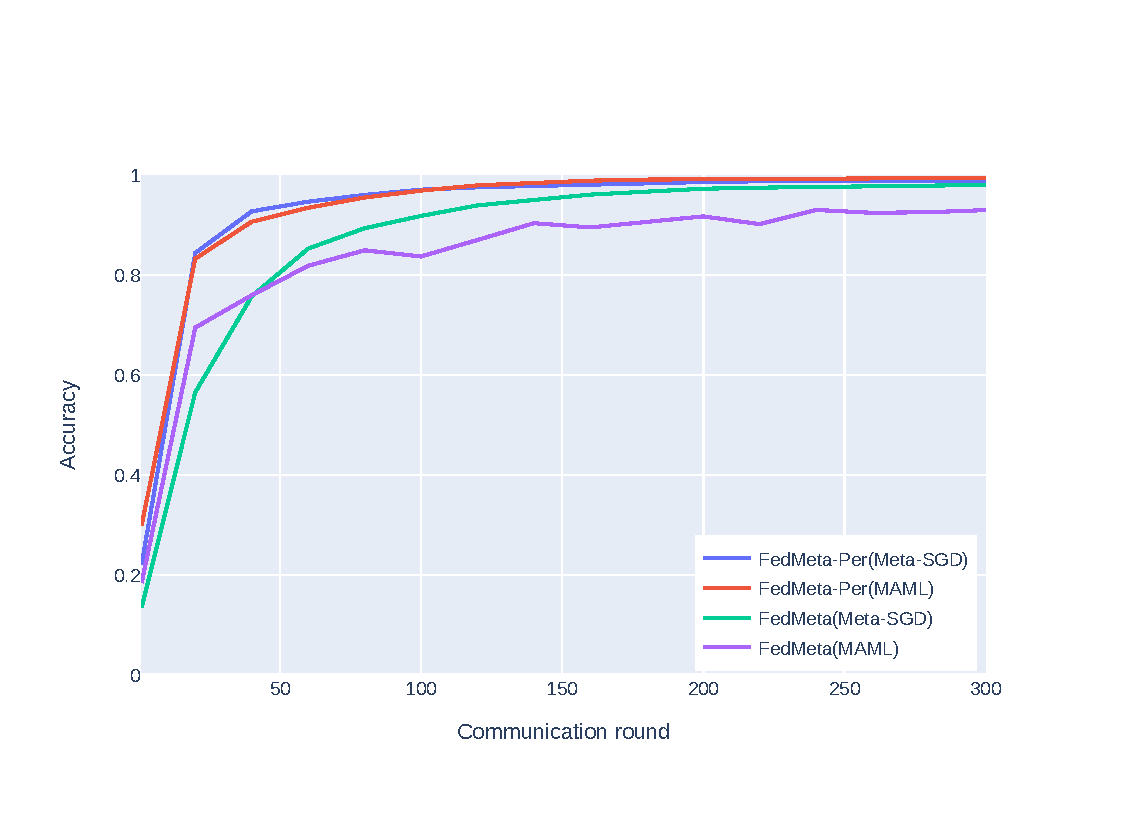
\includegraphics[width=\linewidth]{img/mnist_old_metaper.eps}
            \caption{MNIST, local client}\label{mnist_old_metaper}
        \end{subfigure}
        \begin{subfigure}{.49\textwidth}
            \includegraphics[width=\linewidth]{img/mnist_new_metaper.eps}
            \caption{MNIST, new client}\label{mnist_new_metaper}
        \end{subfigure}
    \end{subfigure}
    \begin{subfigure}{\textwidth}
        \centering
        \begin{subfigure}{.49\textwidth}
            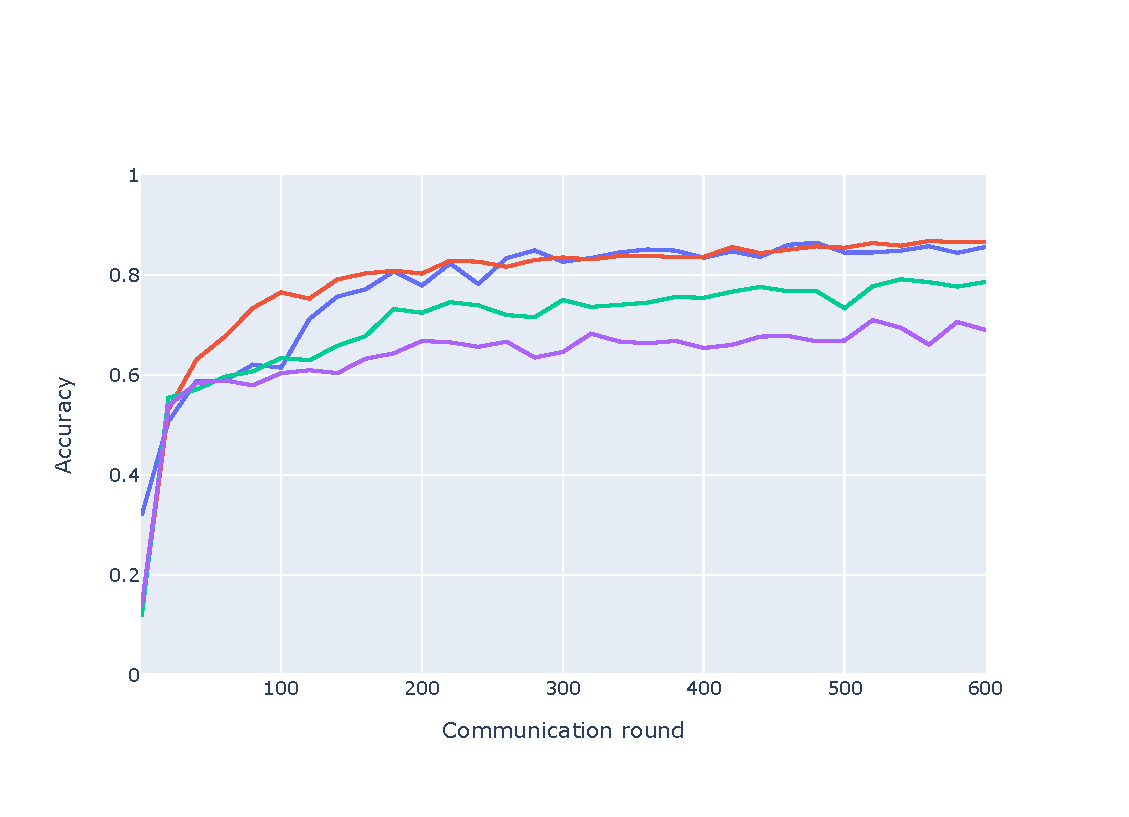
\includegraphics[width=\linewidth]{img/cifar_old_metaper.eps}
            \caption{CIFAR-10, local client}\label{cifar_old_metaper}
        \end{subfigure}
        \begin{subfigure}{.49\textwidth}
            \includegraphics[width=\linewidth]{img/cifar_new_metaper.eps}
            \caption{CIFAR-10, new client}\label{cifar_new_metaper}
        \end{subfigure}
    \end{subfigure}
    \caption{Độ chính xác trên điểm dữ liệu của FedMeta-Per và FedMeta. Kết quả cuối cùng và khả năng hội tụ của FedMeta-Per cao hơn đáng kể so với FedMeta trên người dùng cục bộ. Trên người dùng mới, mặc dù FedMeta-Per đạt giá trị cao hơn, khác biệt trong quá trình hội tụ là không quá lớn.} \label{fig:fedpermeta_vs_fedmeta}
\end{figure}

\begin{figure}[h]
    \centering
    \begin{subfigure}{\textwidth}
        \centering
        \begin{subfigure}{.49\textwidth}
            \includegraphics[width=\linewidth]{img/mnist_old_per.eps}
            \caption{MNIST, local client}\label{fig:mnist_old_per}
        \end{subfigure}
        \begin{subfigure}{.49\textwidth}
            \includegraphics[width=\linewidth]{img/mnist_new_per.eps}
            \caption{MNIST, new client}\label{mnist_new_per}
        \end{subfigure}
    \end{subfigure}
    \begin{subfigure}{\textwidth}
        \centering
        \begin{subfigure}{.49\textwidth}
            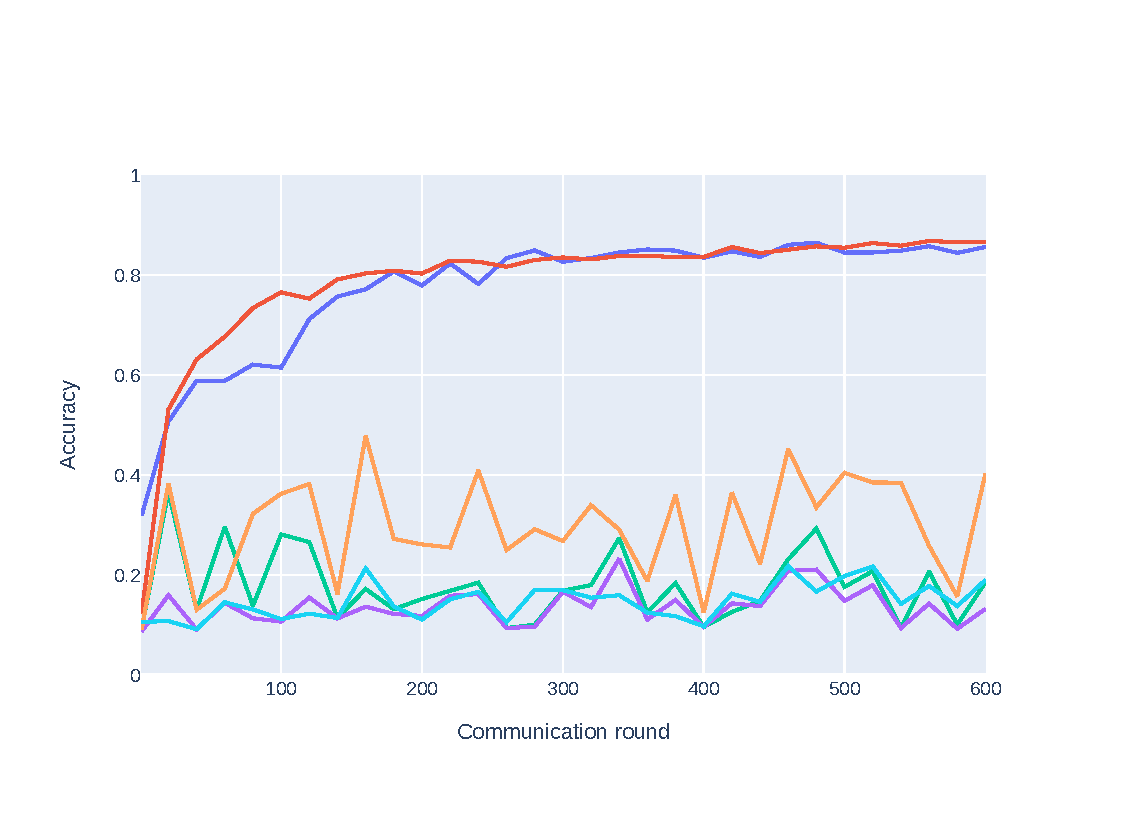
\includegraphics[width=\linewidth]{img/cifar_old_per.eps}
            \caption{CIFAR-10, local client}\label{cifar_old_per}
        \end{subfigure}
        \begin{subfigure}{.49\textwidth}
            \includegraphics[width=\linewidth]{img/cifar_new_per.eps}
            \caption{CIFAR-10, new client}\label{cifar_new_per}
        \end{subfigure}
    \end{subfigure}
    \caption{Độ chính xác trên điểm dữ liệu của FedMeta-Per, FedAvg và FedPer. Khả năng hội tụ cũng như độ chính xác đạt được của FedMeta-Per là vượt trội hơn so với các thuật toán FedAvg và FedPer.} \label{fig:fedpermeta_vs_chicken}
\end{figure}

\textbf{Khả năng cá nhân hoá}. Quan sát độ lệch chuẩn của các thuật toán \codeword{FedMeta}, \codeword{FedAvg} và \codeword{FedPer} trong Bảng \ref{tab:compare}, có thể thấy độ lệch chuẩn trong kết quả của \codeword{FedMeta} nhỏ hơn nhiều so với các thuật toán còn lại. Chứng tỏ tính cá nhân hoá của hệ thống FL đã được cải thiện rất nhiều lần nhờ vào việc huấn luyện theo các thuật toán ML cũng như việc thực hiện fine-tune trên tập support để nắm bắt đặc điểm của một tập dữ liệu mới. Tuy nhiên, như đã đề cập ở trên, khả nằng này hoàn toàn có thể được cải thiện. Bằng các đề xuất mới trong quá trình kiểm thử, \codeword{FedMeta-Per} giúp làm giảm hơn nữa độ lệch chuẩn trên các thang đo. Cụ thể, sau khi kết hợp việc fine-tune mô hình trên tập support của dữ liệu cục bộ và việc duy trì lớp cá nhân hoá tại mỗi máy khách, đối với người dùng cục bộ, độ lệch chuẩn giảm từ 4\% đến 14\% trên CIFAR-10 và từ 1\% đến 5\% trên MNIST trong khi các giá trị trung bình vẫn vượt trội. Trên người dùng mới, các giá trị trung bình cao hơn nhưng độ lệch chuẩn trong một vài trường hợp không thực sự nhỏ hơn các thuật toán trước đó. Điều này là do các lớp phần riêng trong mạng học sâu của người dùng mới chưa thực sự khớp với người dùng đó. Tuy nhiên, theo thời gian, khi người dùng mới tham gia vào một hoặc một vài bước huấn luyện cục bộ, họ sẽ tự xây dựng được các lớp phần riêng tốt cho bản thân, dẫn đến việc các thang đo đạt giá trị tương đương người dùng cũ.

\section{Conclusion}

Qua quá trình nghiên cứu, chúng tôi kết hợp các thuật toán ML và các kỹ thuật PL vào hệ thống FL, nhằm cải thiện độ chính xác cũng như khả năng cá nhân hoá cho từng người dùng của hệ thống trên dữ liệu non-IID. Bằng thực nghiệm, chúng tôi chứng minh được tính hiệu quả của thuật toán đề xuất \codeword{FedMeta-Per} so với các thuật toán \codeword{FedAvg}, \codeword{FedPer}, \codeword{FedMeta} trên 50 người dùng với hai tập dữ liệu CIFAR-10 và MNIST. Trong đó, có thể giải thích việc đạt được kết quả cao dựa vào hai yếu tố mang tính thừa kế: (1) - Khả năng thích ứng nhanh trên tập dữ liệu mới của thuật toán đề xuất thừa hưởng từ các thuật toán ML, (2) - Khả năng cá nhân hóa cao cho từng người dùng kế thừa từ các lớp cá nhân hóa của PL và việc fine-tune dữ liệu của ML.

Trong tương lai, các thuật toán ML theo hướng tối ưu hai cấp độ (\codeword{FO-MAML} \cite{finn2017model}, \codeword{iMAML} \cite{rajeswaran2019meta}, \codeword{Reptile}) có thể được tích hợp thêm vào hệ thống. Việc tìm kiếm và phân cụm người dùng sao cho mỗi người dùng tìm được bộ tham số phần riêng tốt nhất cũng nên được nghiên cứu thêm để tăng hiệu suất của hệ thống. Ngoài ra, vấn đề về bảo mật thông tin giữa máy chủ và máy khách cũng nên được xét đến để hệ thống trở nên thực tiễn hơn.

% \begin{figure}[H]
%     \includegraphics[width=\textwidth]{img/cifar_new_metaper.eps}
%     \caption{A figure caption is always placed below the illustration. Please note that short captions are centered, while long ones are justified by the macro package automatically.} \label{fig1}
% \end{figure}
%
% the environments 'definition', 'lemma', 'proposition', 'corollary',
% 'remark', and 'example' are defined in the LLNCS documentclass as well.
%
%
% ---- Bibliography ----
%
% BibTeX users should specify bibliography style 'splncs04'.
% References will then be sorted and formatted in the correct style.
%
\bibliographystyle{splncs04}
\bibliography{mybibliography}

\appendix
\section{Experimental Details}
\label{appendix}

\subsection{Datasets}

Ký hiệu $C_{train} = \{c^{train}_1,...,c^{train}_{50}\}$ là tập máy khách dùng trong huấn luyện, $C_{test} = \{c^{test}_1,...,c^{test}_{50}\}$ là tập máy khách dùng trong kiểm thử, $N$ là tổng số điểm dữ liệu, ta có số lượng dữ liệu huấn luyện và kiểm tra lần lượt là:

\begin{equation*}
    N_{train} = \sum_{i=1}^{50} \left|c^{train}_i\right| = 0.75N
\end{equation*}
\begin{equation*}
    N_{test} = \sum_{i=1}^{50} \left|c^{test}_i\right| = 0.25N
\end{equation*}

Trong cài đặt ML, ký hiệu $c^{train}_i = \{\mathcal{D}_{train(i)}^{support}, \mathcal{D}_{train(i)}^{query}\}$, $ c^{test}_i = \{\mathcal{D}_{test(i)}^{support}, \mathcal{D}_{test(i)}^{query}\}$. Ta có số lượng dữ liệu chứa trong tập support và query của tất cả các máy khách lần lượt là:

\begin{equation*}
    N_{train/test(i)}^{support} = \left|\mathcal{D}_{train/test(i)}^{support}\right| = 0.2 \left|c_i^{train/test}\right|
\end{equation*}
\begin{equation*}
    N_{train/test(i)}^{query} = \left|\mathcal{D}_{train/test(i)}^{query}\right| = 0.8 \left|c^{train/test}_i\right|
\end{equation*}

Người dùng $c_j^{test} \in C_{test}$ được gọi là người dùng cục bộ nếu tồn tại người dùng $c_i^{train}\in C_{train}$ sao cho $p\left((x,y)\in c_j^{test}\right) = p\left((x,y)\in c_i^{train}\right)$. Ngược lại, $c_j^{test}$ là người dùng mới nếu $p\left((x,y)\in c_j^{test}\right) \ne p\left((x,y)\in c_i^{train}\right)$ với mọi $c_i^{train}\in C_{train}$.

\subsection{Model Architecture}
\label{model_architecture}

Nghiên cứu sử dụng hai mô hình đơn giản để rút trích đặc trưng và phân lớp dữ liệu cho tập dữ liệu CIFAR-10 và MNIST.

\textbf{CIFAR-10.} Mô hình nhận các ảnh đầu vào có kích thước $(32\times32\times3)$. Hai lớp tích chập (kernel có kích thước $(5\times5)$, số chanel lần lượt là $6$ và $16$) được sử dụng để rút trích đặc trưng. Theo sau mỗi lớp tích chập là một lớp \codeword{MaxPooing} có kích thước $(2\times2)$. Phần phân lớp gồm ba lớp tuyến tính có đầu ra lần lượt là $120$, $84$ và $10$. Các hàm kích hoạt được sử dụng là \codeword{ReLU} và \codeword{Softmax}.

\textbf{MNIST.} Mô hình nhận các ảnh đầu vào đã được làm phẳng có kích thước $(1\times784)$. Sử dụng hai lớp tuyến tính có đầu ra lần lượt là 100 và 10. Các hàm kích hoạt được sử dụng là \codeword{ReLU} và \codeword{Softmax}.

\subsection{Hyper-parameters Searching}

Các siêu tham số của hệ thống FL của nghiên cứu bao gồm: số máy khách tham gia huấn luyện trong một bước huấn luyện toàn cục ($\#clients/round$), số bước huấn luyện cục bộ ($\#epochs$), số bước huấn luyện toàn cục ($\#rounds$), lượng dữ liệu trong một batch dữ liệu ($batch\_size$), số lớp phần riêng đối với các thuật toán sử dụng kỹ thuật PL ($\#per\_layers$) và các siêu tham số học sử dụng trong tối ưu mạng học sâu bằng kỹ thuật mini batch gradient descent.

Để phù hợp cho phần cứng của các máy khách có cấu hình yếu trong kịch bản Horizontal FL, nghiên cứu giới hạn $\#epochs=1$ và $batch\_size=32$. Từ việc khảo sát các thí nghiệm FL của các nghiên cứu gần đây, số máy khách tham gia huấn luyện toàn cục được được chọn lần lượt là 2, 5 và 10 máy. Trong đó, $\#clients/round=5$ cho kết quả cao hơn và tiêu tốn chi phí tính toán ở một mức chấp nhận được.

Đối với các mạng học sâu được cài đặt, việc duy trì một lớp phần chung và một lớp phần riêng cho mạng neuron MNIST là tất nhiên. Với mạng học sâu dùng cho tập CIFAR-10, $\#per\_layers \in \{1,2,3\}$ (tính từ lớp tuyến tính cuối cùng). Kết quả chạy thực nghiệm cho thấy, việc sử dụng lớp tuyến tính cuối cùng làm phần riêng và các lớp học sâu còn lại làm phần chung cho kết quả tốt nhất.

Ngoại trừ siêu tham số học của từng thuật toán, các siêu tham số kể trên đều được giữ cố định trong quá trình huấn luyện. Bảng \ref{tab:fixed_hyper_param} trình bày tóm tắt các giá trị siêu tham số này.

\begin{table}[h]
    \centering
    \caption{Fixed hyper-parameters in FL system}
    \label{tab:fixed_hyper_param}
    % \resizebox{\linewidth}{!}{%
    \begin{tabular}{l|ccccc} 
    \toprule
             & \#clients/round    & \#epochs           & \#rounds & batch\_size         & \multicolumn{1}{l}{\#per\_layers}  \\ 
    \hline
    MNIST    & \multirow{2}{*}{5} & \multirow{2}{*}{1} & 300      & \multirow{2}{*}{32} & \multirow{2}{*}{1}                \\
    CIFAR-10 &                    &                    & 600      &                     &                                   \\
    \bottomrule
    \end{tabular}
    % }
\end{table}

Các siêu tham số học được tìm kiếm trong khoảng $(10^{-5}, 0.01)$ cho từng thuật toán. Kết quả tìm kiếm được trình bày trong Bảng \ref{tab:hyper_param}. Các ô để trống biểu thị việc không tìm được siêu tham số để mô hình hội tụ.

\begin{table}[h]
    \centering
    \caption{Tuning learning rate for algorithms}
    \label{tab:hyper_param}
    % \resizebox{\linewidth}{!}{%
    \begin{tabular}{l|cc} 
    \toprule
    \begin{tabular}[c]{@{}l@{}}\\\end{tabular} & CIFAR-10           & MNIST                                             \\ 
    \hline
    FedAvg, FedAvgMeta                         & -                  & $10^{-5}$                                      \\
    FedPer, FedPerMeta                         & -                  & $10^{-5}$                                      \\
    FedMeta(MAML) ($\alpha,\beta$)             & $(0.01, 0.001)$    & $(0.001, 0.001)$                                \\
    FedMeta(Meta-SGD)($\alpha,\beta$)          & $(0.001, 0.001)$   & $(0.001, 5\times 10^{-4})$  \\
    FedMeta-Per(MAML)($\alpha,\beta$)          & $(0.001, 0.005)$   & $(0.001, 0.001)$                                \\
    FedMeta-Per(Meta-SGD)($\alpha,\beta$)      & $(0.01,0.01)$      & $(0.001, 5\times 10^{-4})$  \\
    \bottomrule
    \end{tabular}
    % }
\end{table}

% \begin{thebibliography}{8}
% \bibitem{ref_article1}
% Author, F.: Article title. Journal \textbf{2}(5), 99--110 (2016)

% \bibitem{ref_lncs1}
% Author, F., Author, S.: Title of a proceedings paper. In: Editor,
% F., Editor, S. (eds.) CONFERENCE 2016, LNCS, vol. 9999, pp. 1--13.
% Springer, Heidelberg (2016). \doi{10.10007/1234567890}

% \bibitem{ref_book1}
% Author, F., Author, S., Author, T.: Book title. 2nd edn. Publisher,
% Location (1999)

% \bibitem{ref_proc1}
% Author, A.-B.: Contribution title. In: 9th International Proceedings
% on Proceedings, pp. 1--2. Publisher, Location (2010)

% \bibitem{ref_url1}
% LNCS Homepage, \url{http://www.springer.com/lncs}. Last accessed 4
% Oct 2017
% \end{thebibliography}

\end{document}
